

\begin{figure}[h]
\centering
\begin{subfigure}[t]{0.40\textwidth}
    \centering
    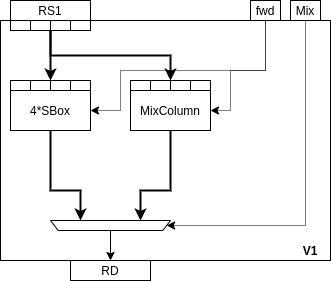
\includegraphics[width=\textwidth]{diagrams/ise-datapath-v1.png}
    \caption{\ISE{1}.}
    \label{fig:ise:design:v1}
\end{subfigure}
\begin{subfigure}[t]{0.40\textwidth}
    \centering
    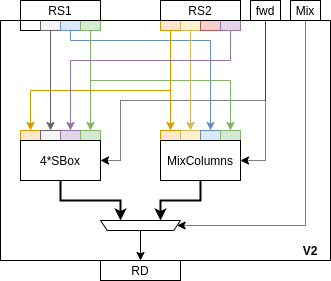
\includegraphics[width=\textwidth]{diagrams/ise-datapath-v2.png}
    \caption{\ISE{2}.}
    \label{fig:ise:design:v2}
\end{subfigure}

\begin{subfigure}[t]{0.40\textwidth}
    \centering
    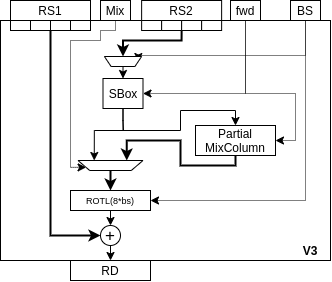
\includegraphics[width=\textwidth]{diagrams/ise-datapath-v3.png}
    \caption{\ISE{3}.}
    \label{fig:ise:design:v3}
\end{subfigure}
\begin{subfigure}[t]{0.40\textwidth}
    \centering
    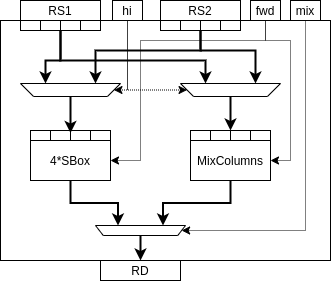
\includegraphics[width=\textwidth]{diagrams/ise-datapath-v5.png}
    \caption{\ISE{5}.}
    \label{fig:ise:design:v5}
\end{subfigure}
\caption{
A block diagram for each ISE variant, illustrating the associated AES functional unit.
}
\label{fig:ise:design}
\end{figure}

% -----------------------------------------------------------------------------
